\chapter{User Interface analysis}
\label{UIA}
In this chapter we describe our decisions and present our analysis and
arguments regarding possible features that we find might have been interesting
to have implemented in our \class{Map Of Denmark} program.

\section{User interface as a whole}
\label{UIA-UIW}
When we designed the first version of the graphical user interface in the first
part of the project, we decided to make a window inside of the graphical user
interface where the actual map should be displayed. We chose to have this
window placed on the right side of our graphical user interface and interaction
with the user mainly placed on the left.

We believe that this is a simple way of representing a user interface for a map.
A lot of software use a menu bar with dropdown menus for selecting different
functions. When we designed our outline for the graphical user interface, we did
not design it with a huge amount of functions in mind. 

The features that we have implemented in this version can easily fit in our
simple user interface, but if features like searching for roads or other
features are included, then space and overview may become an issue on the left side.

If new features are included, we feel it would be beneficial to let the main
window change when different feature types are selected.

Below is a screenshot of our user interface. How to use it will be
explained in the \class{\nameref{MAN}} on page \pageref{MAN}.

\begin{figure}[!ht]
\centering
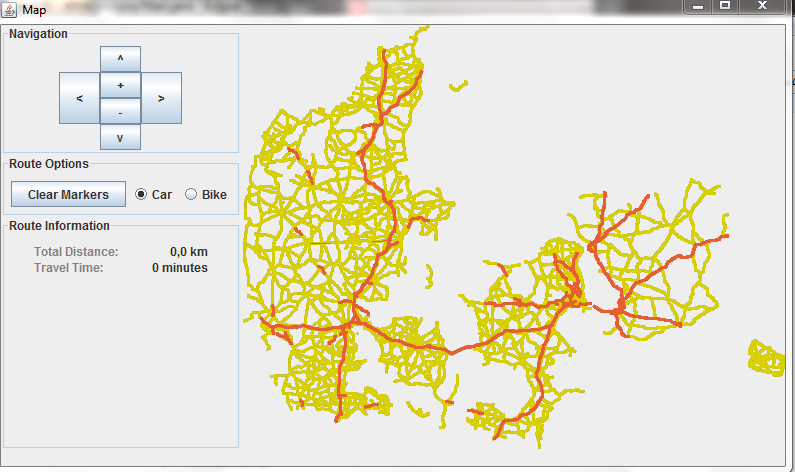
\includegraphics[width=1\linewidth]{images/PictureOfUI}
\caption{Screenshot of GUI}
\label{UIA-UIW-PIC}
\end{figure}

\section{Interesting features}
\label{UIA-IF}
This section presents some of the interesting features we have implemented.
\subsection{Zoom}
\label{UIA-IF-Z}
We have a few options for zooming in and out on the map. As described in
section \ref{BG-R} \class{\nameref{BG-R}} on page \pageref{BG-R}, it
was required that we made it possible to zoom by dragging a box around the part 
of the map the user wants to look closer at.

In addition to the option of using the mouse to zoom, we have implemented a
zoom-in and out function on the GUI and a hotkey for zooming out to the original
zoom level. We made the original zoom function a hotkey only because we did not
want to have too many buttons on the left side. We considered making it a menu bar
item, but we did not manage to get it into this version.

We felt we really needed a zoom out function, so users do not need to close the
program and start it again, when the user wants to view the map further zoomed
out. A combination of the zoom in and out functions helps the user a lot when
navigating the map.

We have limited how far a user can zoom in and out. If the user tries to zoom
out further than the original zoom level, the view will default to the original
zoom level. If the user attempts to zoom in too far compared to the models view,
the zoom function will do nothing.
\subsection{Navigation}
\label{UIA-IF-N}
We have made it possible for the user to navigate the map by using the arrow
buttons on the graphical user interface. When one of the buttons are pressed,
the ``view'' will move in the direction specified by the button. While it was
not specified as a requirement for the project, we felt it was a necessity to
implement at least basic navigation functionality.

Like we did with the two zoom functionalities, we have limited how far a user
can move around the map. If the user moves too far outside the map, the move
function will not do anything.
\subsection{Hotkeys}
\label{UIA-IF-H}
We have implemented hotkeys for all the buttons on the graphical user interface
plus an additional for zooming back to the original zoom level. When we
discussed the benefits of hotkeys, we felt it was important for experienced users of the
software should have a less cumbersome time navigating the map. 

At first we just had hotkeys for the clearing of markers (mentioned in section
\ref{UIA-IF-M}) and zooming out to the original zoom level, but we later added
the hotkeys for the rest of the functionalities. If more features are added in a
future version, it would be important for us that a hotkey were provided, if at
all possible.

\subsection{Route planning and markers}
\label{UIA-IF-M}
Part of the requirements for the project was to provide the user with a way to
get the fastest or shortest route from one point to another. We accomplish this
by putting a ``marker'' at the spot where the user clicks with the mouse. The
marker shows which number in the sequence of markers it is. This will change 
if a marker is removed. Originally we had ``pins'' instead of markers, but we 
changed it, as we felt the pins we had were a bit large.

We have made it possible to place more than the two markers the project
requirements asks for. If the user places more than two markers, the software
will find the shortest route between 1 -> 2 and 2 -> 3 and so on. This was cheap for
us to implement, and we felt it added a nice touch to our program. 

We have implemented two methods of removing pins from the map. We have assigned
a hotkey to the graphical user interface button ``Clear Markers'', which removes 
all the markers from the map. The other way of removing pins is by clicking on
them. This functionality is both intuitive and confusing at the same time. It is
intuitive to click the marker you have just placed if you want to remove it, but
it is not obvious in our interface. We believe that it is enough to have the
``clear all markers'' functionality for those who do not find it intuitive to
click markers to remove them, and for the users that do find it intuitive, we
offer them an easy way to undo a missclick.

\subsection{Bike/car}
\label{UIA-IF-BC}
Another interesting feature in our \class{Map of Denmark} project is the option
to switch between bike and car routes. The user interface will start with car
selected when the program starts.

Whenever a route is calculated, it will display the length and the estimated
travel time on the left part of the user interface. When the bike option is selected, 
it recalculates the route for a bike, without visiting highways and other roads 
that bikes cannot or are not allowed to drive on. If the user switches back to the 
car mode, it recalculates the route again, but not visiting small paths and other 
roads where a car is not allowed to drive. The estimated travel time is also 
recalculated. The user does not need to have planned a route before he/she 
changes the type of transportation.

We have implemented this to help our software target a wider group of people.
The bike/car options were a bit costly to implement, but we categorized it as a
very beneficial feature and we did not feel we could leave it out.

\section{Features not implemented}
\label{UIA-NI}
This section presents some of the features we chose not to implement.
These features are not in the final program, because we did not feel there were
compelling arguments for implementing them.

Features that we wanted to implement, but did not make it into the final version,
will be discussed in chapter \ref{PRC} \class{\nameref{PRC}} on page
\pageref{PRC}.

\subsection{Choice of roads to be displayed}
\label{UIA-NI-CRD}
We chose not to implement the option of selecting which roads to be displayed.
In a sense our program already does this by showing more detail the further
zoomed in the map is. It could become very confusing if the user had the option
of selecting roads, because the graphical user interface could become very
cluttered, if all the roads were listed.

We felt that our gradually increasing level of detail is enough, and if the user were 
to enable all types of roads at once, the map could get quite slow and cumbersome 
to use.

If we were to implement something like this, it would be to give the user the choice 
which types of roads should be included in the route planning - ferries, highways, 
bridges etc. This could be too big a choice for the user to handle though. The
user might doubt if he or she has chosen to best options for finding a route.

\subsection{Smooth scrolling}
\label{UIA-NI-SS}
We made an attempt to let the keyboard arrows scroll smoothly over the map, but
we could not get it to work fast enough, and the user would experience
lockups and an unresponsive interface. A solution to this would
be to save map as images that you can scroll across - this would be faster, but
would require more disk space. Because we store the data the way we do, which 
forces us to draw every line individually every time the user moves the viewport, 
we cannot do this fast enough.

In the end, we decided the benefits of the smooth scrolling were not large enough
for us to spend a lot of time implementing this feature. The cost of changing that  
much way we draw the roads, was simply too high compared to the benefits.

\subsection{Dynamic route finding}
\label{UIA-NI-DRF}
In the final project description, a dynamic route finding feature was
suggested. If we had implemented the suggested dynamic route finding feature, a
user would be able to mark a spot and then whenever he moused over a node on the
map, it would show the route instantly.

We considered implementing this as we thought it was a
nice feature to have, but it conflicted with the algorithm we use for
calculating the route. More about the algorithms can be read in section
\ref{IMPL-DVA} \class{\nameref{IMPL-DVA}} on page \pageref{IMPL-DVA}.
